%% Model-fitting report: data, reporting-delay correction, likelihood, estimation, diagnostics, sensitivity, code.
\documentclass[10pt,a4paper]{article}
\usepackage[T1]{fontenc}\usepackage[utf8]{inputenc}\usepackage{lmodern,microtype}
\usepackage[margin=2.2cm]{geometry}
\usepackage{amsmath,amssymb,booktabs,graphicx,xcolor,caption,enumitem,float,listings}
\usepackage[numbers,sort&compress]{natbib}
\usepackage[colorlinks,linkcolor=blue!50!black,citecolor=blue!50!black,urlcolor=blue!50!black]{hyperref}
% AUTO-GENERATED by R/07_figures_tables.R -- do not edit
\newcommand{\ReEightyFive}{0.89 (0.82 to 0.95)}
\newcommand{\ReEightyThree}{0.74 (0.68 to 0.79)}
\newcommand{\ReFiftyFive}{0.95 (0.86 to 1.02)}
\newcommand{\ReFiftyThree}{0.87 (0.80 to 0.93)}
\newcommand{\ReHundredFive}{0.83 (0.77 to 0.88)}
\newcommand{\ReHundredThree}{0.60 (0.55 to 0.64)}
\newcommand{\ReMedEightyFive}{0.89}
\newcommand{\ReMedEightyThree}{0.74}
\newcommand{\ReMedFiftyFive}{0.95}
\newcommand{\ReMedFiftyThree}{0.87}
\newcommand{\ReMedHundredFive}{0.83}
\newcommand{\ReMedHundredThree}{0.60}
\newcommand{\aIsoFive}{58\%}
\newcommand{\aIsoSeven}{50\%}
\newcommand{\aIsoThree}{70\%}
\newcommand{\avertEightyFive}{22,821 (5,312 to 90,341)}
\newcommand{\avertEightyThree}{27,786 (7,467 to 102,382)}
\newcommand{\avertFiftyFive}{15,595 (3,200 to 64,632)}
\newcommand{\avertFiftyThree}{23,490 (5,527 to 93,061)}
\newcommand{\avertHundredFive}{26,062 (6,700 to 98,336)}
\newcommand{\avertHundredThree}{29,088 (8,364 to 103,935)}
\newcommand{\avertedEightyFive}{22,821}
\newcommand{\avertedEightyThree}{27,786}
\newcommand{\avertedFiftyFive}{15,595}
\newcommand{\avertedFiftyThree}{23,490}
\newcommand{\avertedHundredFive}{26,062}
\newcommand{\avertedHundredThree}{29,088}
\newcommand{\baseCases}{31,089 (9,845 to 107,831)}
\newcommand{\baseCasesMed}{31,089}
\newcommand{\cfrAssumed}{48\%}
\newcommand{\critReEightyFive}{1.13}
\newcommand{\critReEightyThree}{1.36}
\newcommand{\critReFiftyFive}{1.06}
\newcommand{\critReFiftyThree}{1.15}
\newcommand{\critReHundredFive}{1.20}
\newcommand{\critReHundredThree}{1.67}
\newcommand{\crudeCFR}{48\%}
\newcommand{\deathsEightyFive}{11,023}
\newcommand{\deathsEightyThree}{13,421}
\newcommand{\deathsFiftyFive}{7,532}
\newcommand{\deathsFiftyThree}{11,346}
\newcommand{\deathsHundredFive}{12,588}
\newcommand{\deathsHundredThree}{14,050}
\newcommand{\delayHalf}{7}
\newcommand{\delayMean}{8.5}
\newcommand{\delayNinety}{15}
\newcommand{\desolveVersion}{1.40}
\newcommand{\durEightyFive}{24}
\newcommand{\durEightyThree}{9}
\newcommand{\durFiftyFive}{53}
\newcommand{\durFiftyThree}{22}
\newcommand{\durHiEightyFive}{53}
\newcommand{\durHiEightyThree}{14}
\newcommand{\durHiFiftyFive}{$>$60}
\newcommand{\durHiFiftyThree}{49}
\newcommand{\durHiHundredFive}{21}
\newcommand{\durHiHundredThree}{7}
\newcommand{\durHundredFive}{13}
\newcommand{\durHundredThree}{5}
\newcommand{\durLoEightyFive}{14}
\newcommand{\durLoEightyThree}{7}
\newcommand{\durLoFiftyFive}{21}
\newcommand{\durLoFiftyThree}{13}
\newcommand{\durLoHundredFive}{9}
\newcommand{\durLoHundredThree}{4}
\newcommand{\fitAReAfter}{1.04 (0.98 to 1.07)}
\newcommand{\fitAReAfterMed}{1.04}
\newcommand{\fitAReBefore}{1.19 (1.13 to 1.27)}
\newcommand{\fitAReBeforeMed}{1.19}
\newcommand{\fitAacf}{0.27}
\newcommand{\fitAcover}{96\%}
\newcommand{\fitAdAIC}{14.5}
\newcommand{\fitAincEnd}{63 (55 to 71)}
\newcommand{\fitAincEndMed}{63}
\newcommand{\fitApGrow}{0.95}
\newcommand{\fitArAfter}{0.004 ($-$0.001 to 0.006)}
\newcommand{\fitArBefore}{0.017 (0.011 to 0.023)}
\newcommand{\fitAtc}{5 July}
\newcommand{\fitAtcRange}{28 June to 2 August}
\newcommand{\fitBReAfter}{1.00 (0.93 to 1.06)}
\newcommand{\fitBReAfterMed}{1.00}
\newcommand{\fitBReBefore}{1.20 (1.16 to 1.25)}
\newcommand{\fitBReBeforeMed}{1.20}
\newcommand{\fitBacf}{0.01}
\newcommand{\fitBcover}{95\%}
\newcommand{\fitBdAIC}{15.4}
\newcommand{\fitBincEnd}{83 (68 to 100)}
\newcommand{\fitBincEndMed}{83}
\newcommand{\fitBpGrow}{0.56}
\newcommand{\fitBrAfter}{0.000 ($-$0.006 to 0.006)}
\newcommand{\fitBrBefore}{0.018 (0.014 to 0.022)}
\newcommand{\fitBtc}{24 July}
\newcommand{\fitBtcRange}{18 July to 7 August}
\newcommand{\fracIsoBase}{51\%}
\newcommand{\fracIsoEightyFive}{59\%}
\newcommand{\fracIsoEightyThree}{71\%}
\newcommand{\fracIsoFiftyFive}{59\%}
\newcommand{\fracIsoFiftyThree}{71\%}
\newcommand{\fracIsoHundredFive}{59\%}
\newcommand{\fracIsoHundredThree}{71\%}
\newcommand{\meanSep}{86}
\newcommand{\nConfirmed}{7,200}
\newcommand{\nDeaths}{3,475}
\newcommand{\nDraws}{1,000}
\newcommand{\nIntervals}{96}
\newcommand{\nOnsetCases}{4,724}
\newcommand{\nOnsetDays}{105}
\newcommand{\nPRCC}{1,500}
\newcommand{\nRetro}{272}
\newcommand{\nStoch}{500}
\newcommand{\nVarDraws}{300}
\newcommand{\nVariants}{17}
\newcommand{\nVintages}{55}
\newcommand{\nhIncMax}{84}
\newcommand{\nhIncMin}{81}
\newcommand{\nhRMax}{0.0009}
\newcommand{\nhRMin}{$-$0.0005}
\newcommand{\pEndBaseSixty}{0.12}
\newcommand{\pEndBaseTwentyFour}{0.01}
\newcommand{\pEndYearFiveEightyFive}{0.99}
\newcommand{\pEndYearFiveEightyThree}{1.00}
\newcommand{\pEndYearFiveFiftyFive}{0.58}
\newcommand{\pEndYearFiveFiftyThree}{0.99}
\newcommand{\pEndYearFiveHundredFive}{1.00}
\newcommand{\pEndYearFiveHundredThree}{1.00}
\newcommand{\pEndYearOneEightyFive}{0.01}
\newcommand{\pEndYearOneEightyThree}{0.90}
\newcommand{\pEndYearOneFiftyFive}{0.00}
\newcommand{\pEndYearOneFiftyThree}{0.01}
\newcommand{\pEndYearOneHundredFive}{0.33}
\newcommand{\pEndYearOneHundredThree}{1.00}
\newcommand{\pEndYearTwoEightyFive}{0.52}
\newcommand{\pEndYearTwoEightyThree}{1.00}
\newcommand{\pEndYearTwoFiftyFive}{0.05}
\newcommand{\pEndYearTwoFiftyThree}{0.60}
\newcommand{\pEndYearTwoHundredFive}{0.99}
\newcommand{\pEndYearTwoHundredThree}{1.00}
\newcommand{\pReBaseBelow}{0.44}
\newcommand{\pReBelowEightyFive}{1.00}
\newcommand{\pReBelowEightyThree}{1.00}
\newcommand{\pReBelowFiftyFive}{0.94}
\newcommand{\pReBelowFiftyThree}{1.00}
\newcommand{\pReBelowHundredFive}{1.00}
\newcommand{\pReBelowHundredThree}{1.00}
\newcommand{\pctEightyFive}{73 (55 to 84)}
\newcommand{\pctEightyThree}{89 (76 to 95)}
\newcommand{\pctFiftyFive}{50 (33 to 62)}
\newcommand{\pctFiftyThree}{75 (57 to 86)}
\newcommand{\pctHundredFive}{84 (68 to 93)}
\newcommand{\pctHundredThree}{94 (85 to 98)}
\newcommand{\pctMedEightyFive}{73\%}
\newcommand{\pctMedEightyThree}{89\%}
\newcommand{\pctMedFiftyFive}{50\%}
\newcommand{\pctMedFiftyThree}{75\%}
\newcommand{\pctMedHundredFive}{84\%}
\newcommand{\pctMedHundredThree}{94\%}
\newcommand{\popAtRisk}{4,392,200}
\newcommand{\posJun}{22.6}
\newcommand{\posSep}{17.1}
\newcommand{\prccGrowthRate}{0.42}
\newcommand{\prccInfectiousPeriod}{0.10}
\newcommand{\prccIsolationDelay}{0.94}
\newcommand{\prccIsolationEffectiveness}{$-$0.80}
\newcommand{\prccLatentPeriod}{0.27}
\newcommand{\prccStartingIncidence}{0.17}
\newcommand{\rVersion}{4.3.3 (2024-02-29)}
\newcommand{\rYear}{2024}
\newcommand{\shareOnset}{66\%}
\newcommand{\stochBase}{32,114}
\newcommand{\stochEndBase}{0.31}
\newcommand{\stochEndFive}{0.73}
\newcommand{\stochEndThree}{0.86}
\newcommand{\stochFive}{8,904}
\newcommand{\stochRatioMax}{1.09}
\newcommand{\stochRatioMin}{1.00}
\newcommand{\stochRedFive}{72\%}
\newcommand{\stochRedThree}{89\%}
\newcommand{\stochThree}{3,588}
\newcommand{\testsJun}{168}
\newcommand{\testsSep}{494}
\newcommand{\valCumMod}{10,981}
\newcommand{\valCumObs}{10,274}
\newcommand{\valErrLong}{23\%}
\newcommand{\valErrShort}{35\%}
\newcommand{\valInsideLong}{inside}
\newcommand{\valInsideShort}{outside}
\newcommand{\valModLong}{3,781}
\newcommand{\valModLongCI}{3,781 (2,796 to 4,991)}
\newcommand{\valModShort}{1,236}
\newcommand{\valNaiveErrLong}{24\%}
\newcommand{\valObsLong}{3,074}
\newcommand{\valObsShort}{916}
\newcommand{\valPredLongHi}{5,126}
\newcommand{\valPredLongLo}{2,743}
\newcommand{\valRateObsLong}{67}
\newcommand{\valRateObsShort}{61}
\newcommand{\varBaseFourFive}{$-$67 ($-$98 to $-$37)}
\newcommand{\varBaseFourThree}{80 (63 to 90)}
\newcommand{\varCondFive}{83}
\newcommand{\varCondIso}{6\%}
\newcommand{\varCondThree}{93}
\newcommand{\varErlangTenFive}{78}
\newcommand{\varErlangTenThree}{91}
\newcommand{\varErlangThreeFive}{77}
\newcommand{\varFitABase}{51,067}
\newcommand{\varFitAFive}{82}
\newcommand{\varFitAThree}{94}
\newcommand{\varFiveMax}{84}
\newcommand{\varFiveMin}{56}
\newcommand{\varGrowthHiBase}{92,275}
\newcommand{\varGrowthHiFive}{84}
\newcommand{\varGrowthHiThree}{96}
\newcommand{\varGrowthLoBase}{11,750}
\newcommand{\varGrowthLoFive}{56}
\newcommand{\varGrowthLoThree}{77}
\newcommand{\varIncHiFive}{73}
\newcommand{\varIncLoFive}{73}
\newcommand{\varPopFive}{73}
\newcommand{\varRampNinetyFive}{62}
\newcommand{\varRampNinetyThree}{81}
\newcommand{\varRampNinetyUiLo}{40}
\newcommand{\varRampThirtyFive}{69}
\newcommand{\varRampThirtyThree}{86}
\newcommand{\varThreeMax}{96}
\newcommand{\varThreeMin}{77}

\graphicspath{{../figures/}}
\captionsetup{font=small,labelfont=bf}\setlist{nosep,leftmargin=1.3em}\setlength{\parskip}{3pt}\setlength{\parindent}{0pt}
\newcommand{\Rt}{R_{\mathrm{e}}}
\lstset{language=R,basicstyle=\ttfamily\fontsize{6.4}{7.4}\selectfont,breaklines=true,numbers=left,numberstyle=\tiny\color{gray},numbersep=4pt,frame=single,rulecolor=\color{gray!50},commentstyle=\color{green!35!black}\itshape,keywordstyle=\color{blue!50!black},showstringspaces=false,columns=fullflexible,keepspaces=true}
\begin{document}
{\Large\bfseries Model fitting report: SEIQR model for the 2026 Bundibugyo outbreak, DRC}\\[3pt]
{\small Team TAUS \;|\; companion to the manuscript \;|\; every number below is generated by \texttt{R/02\_fit.R} and \texttt{R/07\_figures\_tables.R}}

\section{What is fitted and why}
The scenarios need three data-determined inputs: the current growth rate, the current incidence, and the date transmission changed. Case counts cannot identify the natural history, the baseline delay or the isolation effectiveness $\epsilon$; these are fixed (latent period 6.3 d, infectious period 7 d, baseline delay 7 d, $\epsilon=0.8$) and varied afterwards. The fitted quantities are the starting incidence $i_0$ (on 2 May 2026), transmission rates $\beta_1,\beta_2$ before and after a change date $t_c$, and the negative-binomial dispersion $k$ (counting $t_c$, five parameters, against three for constant transmission).

\section{Data}
Fit B (primary): confirmed cases by report date, 2 June--12 September (96 report intervals) from the BVDOutbreakSize streams \citep{bvdoutbreaksize2026}. The 22 July harmonisation step (369 reported, 97 new) is replaced by the printed 97, removing 272 retrospective cases. Fit A (cross-check): confirmed cases by onset date from SitRep 121 (25 May--6 September, 105 days; about \shareOnset{} of confirmed cases have a recorded onset), corrected for right-truncation. Suspected cases, bed capacity and treatment-centre streams stop or change definition and are not used.

\section{Reporting-delay correction}
Each SitRep republishes the onset curve, so the share of an onset day's final count visible $L$ days later can be measured over \nVintages{} vintages (final = counts at least 28 days old in the latest vintage). A Weibull cumulative distribution $c(L)=1-\exp\{-((L+0.5)/s)^\kappa\}$ fits it: half of cases visible after \delayHalf{} days, 90\% after \delayNinety{} days, mean \delayMean{} days. This explains the apparent collapse of the onset curve in the last three weeks (Fig.~\ref{fig:fit}a,b).

\section{Model, likelihood and estimation}
Model~\eqref{eq:m} is the SEIQR system with $\lambda=\beta[I+(1-\epsilon)Q]/N$:
\begin{equation}\dot S=-\lambda S,\;\dot E=\lambda S-\sigma E,\;\dot I=\sigma E-(\tau+\gamma)I,\;\dot Q=\tau I-\gamma Q,\;\dot R=\gamma(I+Q).\label{eq:m}\end{equation}
Symptomatic incidence is $i(d)=\sigma E(d)$. Observations are negative binomial with mean $\mu$ and variance $\mu+\mu^2/k$. In Fit A, $\mu_d=c(L_d)\,i(d)$. In Fit B the expected count over a report interval is the incidence convolved with the daily delay probabilities $c(L)-c(L-1)$ and summed over the interval's days. The transmission rate changes from $\beta_1$ to $\beta_2$ on day $t_c$. Maximum likelihood used Nelder--Mead from several starts; $t_c$ was profiled on a 5-day grid and refined to 1 day. Uncertainty draws sample $t_c$ with weights proportional to the profile likelihood and the other parameters from the Hessian-based multivariate normal at that $t_c$. $\Delta$AIC compares with constant transmission.

\section{Results}
\begin{table}[H]\centering\scriptsize\caption{Fitted parameters (median and 95\% uncertainty interval), $\epsilon=0.8$, baseline delay 7 d; growth rates per day.}
\resizebox{\textwidth}{!}{\begin{tabular}{@{}lccccccc@{}}
\toprule
Fit & Growth rate before (/d) & Growth rate after (/d) & $R_e$ before & $R_e$ after & Change date (95\% interval) & $\Delta$AIC & Incidence 12 Sep (/d) \\
\midrule
A: onset curve & 0.0169 (0.0112--0.0234) & 0.0040 ($-$0.0015 to 0.0065) & 1.19 (1.13--1.27) & 1.04 (0.98--1.07) & 5 July (28 June--2 August) & 14.5 & 63 (55--71) \\
B: report date & 0.0177 (0.0140--0.0216) & 0.0004 ($-$0.0062 to 0.0058) & 1.20 (1.16--1.25) & 1.00 (0.93--1.06) & 24 July (18 July--7 August) & 15.4 & 83 (68--100) \\
\bottomrule
\end{tabular}
}\end{table}
A change in transmission was strongly supported ($\Delta$AIC \fitAdAIC{} for Fit A, \fitBdAIC{} for Fit B). In Fit B growth fell from \fitBrBefore{} to \fitBrAfter{} per day around \fitBtc{} (interval \fitBtcRange), i.e.\ $\Rt$ from \fitBReBefore{} to \fitBReAfter. The model incidence on 12 September was \fitBincEnd{} per day (Fit A: \fitAincEnd, covering only cases with an onset date).
\begin{figure}[H]\centering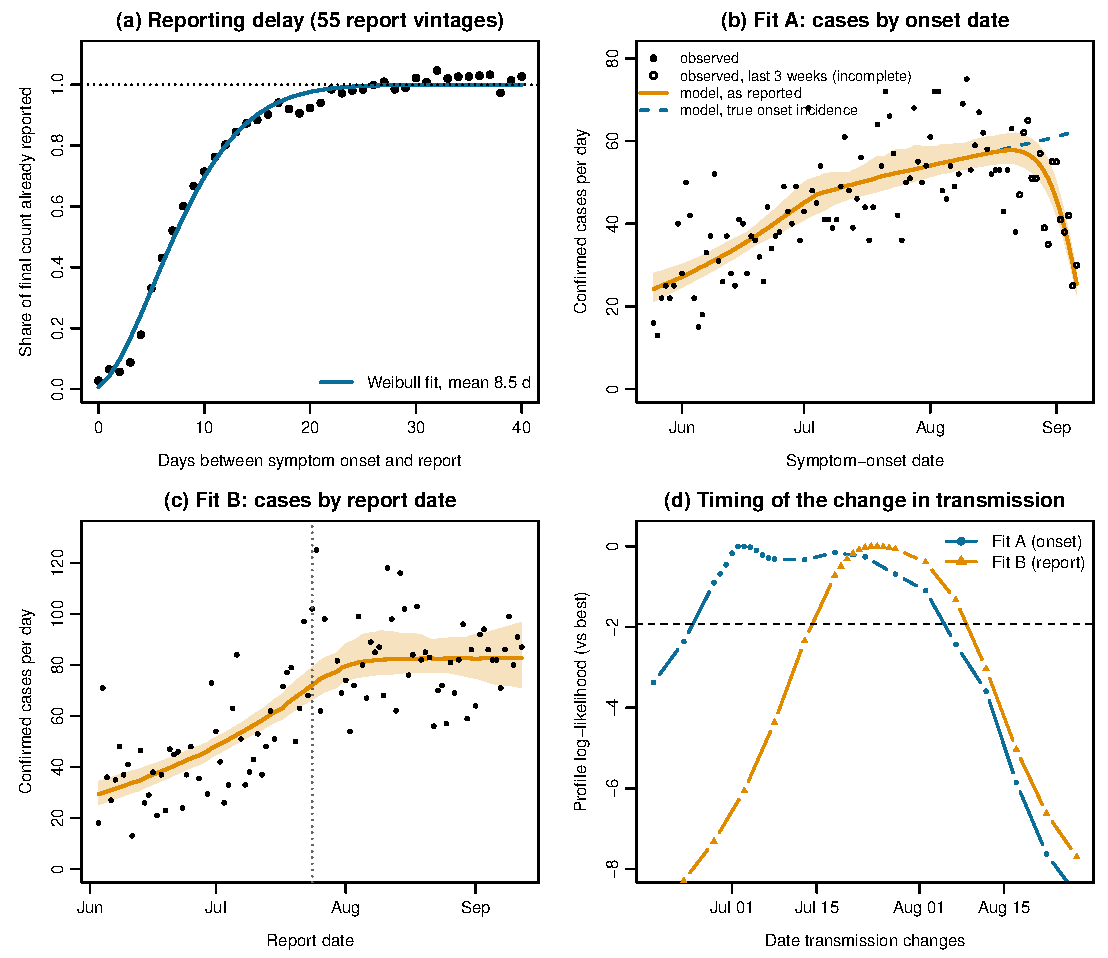
\includegraphics[width=0.95\textwidth]{fig2_fit.pdf}\caption{Fitting outcome. (a) Reporting-delay curve from \nVintages{} vintages. (b) Fit A with right-truncation correction. (c) Fit B, report-date counts with the change date. (d) Profile log-likelihood for the change date.}\label{fig:fit}\end{figure}

\section{Diagnostics}
95\% negative-binomial predictive intervals covered \fitAcover{} (Fit A) and \fitBcover{} (Fit B) of observations; lag-1 residual autocorrelation was \fitAacf{} and \fitBacf. Refitting Fit B at the four corners of the natural-history ranges changed the post-change growth rate only between \nhRMin{} and \nhRMax{} per day and the 12 September incidence between \nhIncMin{} and \nhIncMax{} (Table~\ref{tab:nh}), so these two quantities are determined by the data rather than by the assumed natural history. Because $\beta$ and $\epsilon$ are not separately identifiable, the growth rates are identical for every $\epsilon$ (Table~\ref{tab:eff}). Testing expanded from \testsJun{} to \testsSep{} samples per day while positivity fell from \posJun\% to \posSep\% (Table~\ref{tab:pos}), so the plateau is not simply a laboratory-capacity ceiling.
\begin{table}[H]\centering\small\caption{Fit B refitted at extreme natural-history values.}\label{tab:nh}\begin{tabular}{@{}cccccc@{}}
\toprule
Latent (d) & Infectious (d) & Neg.\ log-lik. & $\beta$ after & Growth rate after (/d) & Incidence 12 Sep (/d) \\
\midrule
4.0 & 5 & 407.60 & 0.300 & -0.0001 & 81.7 \\
10.1 & 5 & 407.59 & 0.298 & -0.0005 & 81.2 \\
4.0 & 10 & 407.62 & 0.191 & 0.0009 & 83.5 \\
10.1 & 10 & 407.58 & 0.190 & 0.0002 & 82.4 \\
\bottomrule
\end{tabular}
\end{table}
\begin{table}[H]\centering\small\caption{Fit by isolation effectiveness.}\label{tab:eff}\begin{tabular}{@{}clccccc@{}}
\toprule
Fit & Isolation eff. & $\beta$ before & $\beta$ after & Growth after (/d) & $R_e$ before & $R_e$ after \\
\midrule
A & 50\% & 0.235 & 0.201 & 0.0046 & 1.24 & 1.06 \\
B & 50\% & 0.233 & 0.191 & 0.0003 & 1.23 & 1.00 \\
A & 80\% & 0.288 & 0.250 & 0.0044 & 1.21 & 1.05 \\
B & 80\% & 0.286 & 0.238 & 0.0000 & 1.20 & 1.00 \\
A & 100\% & 0.339 & 0.298 & 0.0043 & 1.19 & 1.04 \\
B & 100\% & 0.337 & 0.285 & -0.0003 & 1.18 & 1.00 \\
\bottomrule
\end{tabular}
\end{table}
\begin{table}[H]\centering\small\caption{Testing and positivity by month.}\label{tab:pos}\begin{tabular}{@{}lcccc@{}}
\toprule
Month (2026) & New confirmed cases & Samples analysed & Samples per day & Positivity (\%) \\
\midrule
Jun & 987 & 4,365 & 168 & 22.6 \\
Jul & 1,996 & 9,102 & 294 & 21.9 \\
Aug & 2,512 & 13,373 & 431 & 18.8 \\
Sep & 1,014 & 5,927 & 494 & 17.1 \\
\bottomrule
\end{tabular}
\end{table}

\section{Out-of-sample check}
A forecast using data to 12 September overestimated the next 46 days by \valErrLong{} (model \valModLongCI{} against \valObsLong{} observed; observed inside the interval), and the next 15 days by \valErrShort{} (outside). A constant-rate benchmark erred similarly (\valNaiveErrLong{} at 46 days).

\section{Reproduce}
\texttt{Rscript R/run\_all.R} (about 15 min) runs tests, \texttt{01\_data\_prep.R}, \texttt{02\_fit.R} and the remaining analysis, and \texttt{Rscript R/08\_build\_reports.R} rebuilds this report. Code for the fitting steps follows.

\appendix\clearpage
\section{Code: data preparation (R/01\_data\_prep.R)}\lstinputlisting{../R/01_data_prep.R}
\section{Code: fitting (R/02\_fit.R)}\lstinputlisting{../R/02_fit.R}
\section{Code: shared model functions (R/00\_functions.R)}\lstinputlisting{../R/00_functions.R}
{\footnotesize\bibliographystyle{unsrtnat}\bibliography{../manuscript/references}}
\end{document}
